%========ANÁLISIS DEL MODULO DE COMUNICACIÓN=======

\subsection{Sistema operativo móvil}
Los sistemas operativos para teléfonos inteligentes o sistemas operativos móviles son sistemas operativos que operan teléfonos inteligentes, PDA, tabletas y otros dispositivos móviles. Un sistema operativo permite que estos dispositivos ejecuten aplicaciones y programas, por lo tanto, llevan funciones avanzadas a dispositivos móviles que anteriormente estaban restringidos a computadoras de escritorio. \\

En la figura \ref{fig:grafica_mercadoOS} se muestra una gráfica que indica la participación de mercado global del sistema operativo móvil, en términos de ventas a usuarios finales, de 2009 a 2018. En el segundo trimestre de 2018, el 88\% de los teléfonos celulares vendidos a usuarios finales eran teléfonos con el sistema operativo Android \cite{mercadoOS}. \\

\begin{figure}[htbp!]
	\centering
	\fbox{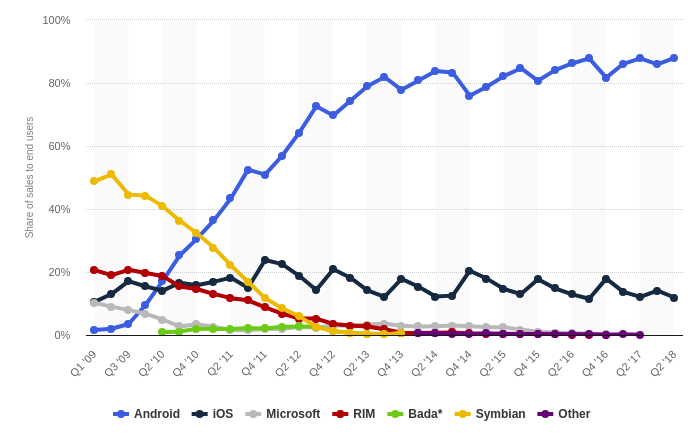
\includegraphics[width=0.9\textwidth]{Analisis/imagenes/mercadoOS.png}}
	\caption{Sistemas operativos móviles en el mercado global. Statista (2018).}
	\label{fig:grafica_mercadoOS}
\end{figure}

A pesar de existir varios sistemas operativos móviles como: Microsoft, Symbian, RIM, Android, iOS, entre otros, son dos los que actualmente abarcan casi la totalidad del mercado: Android e iOS, por lo que para el desarrollo de la aplicación móvil únicamente se considerarán éstos dos. \\


En la figura \ref{fig:mercadoMexico} se muestra el porcentaje de dispositivos vendidos con sistema operativo Android (81.45\%) e iOS (17.34\%) en México, indicando una gran diferencia entre la cantidad de dispositivos con estos sistemas operativos vendidos entre octubre de 2017 y septiembre de 2018. \\

\begin{figure}[htbp!]
	\centering
	\fbox{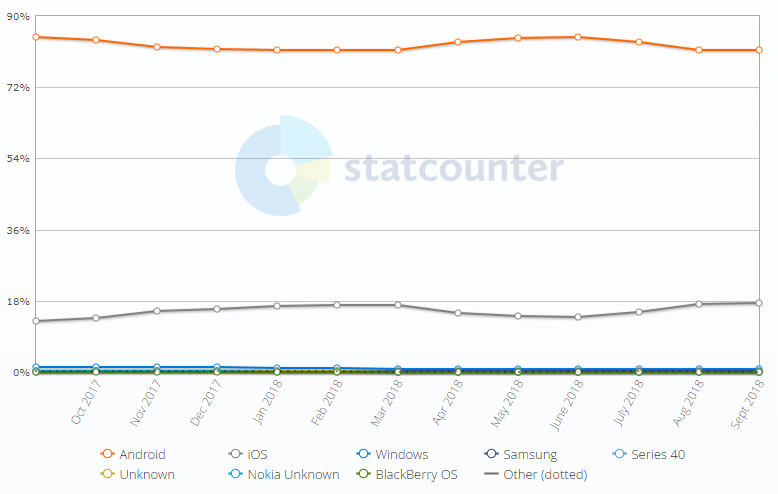
\includegraphics[width=0.9\textwidth]{Analisis/imagenes/mercadoMexico.png}}
	\caption{Sistemas operativos móviles en México. Statcounter (2018).}
	\label{fig:mercadoMexico}
\end{figure}

Debido a la popularidad del sistema operativo Android en México, se decidió desarrollar la aplicación para este sistema operativo y así lograr que pueda ser utilizado por un mayor número de personas. Por lo tanto la aplicación móvil será desarrollada para el sistema operativo Android y se buscará que sea compatible con la versión más reciente, Pie 9.0 y las versiones Oreo 8.1, Nougat 7.0 y 7.1, y Marshmallow 6.0 con la finalidad de que sea compatible con el mayor porcentaje de dispositivos y poder realizar pruebas con algún dispositivo físico más fácilmente. \\

\clearpage